\documentclass[aps,longbibliography,english,superscriptaddress,prx]{revtex4-1}
\usepackage[colorlinks=true,urlcolor=blue,citecolor=blue,linkcolor=blue]{hyperref}
\usepackage[T1]{fontenc}
%\usepackage[latin9]{inputenc}
\usepackage{amssymb}
\usepackage{enumitem}
\usepackage{tabularx}
%\usepackage{caption}
\usepackage[plain]{algorithm}
\usepackage{algpseudocode}
\usepackage{rotating}
\usepackage{booktabs}
\usepackage{amsthm}
%\usepackage{unicode-math}
%\usepackage{algorithm}% http://ctan.org/pkg/algorithm
%\usepackage{algpseudocode}% http://ctan.org/pkg/algpseudocode
\usepackage{bbm}
\usepackage{graphicx, subfigure}
\usepackage{amsmath,color}
\usepackage{mathrsfs}
\usepackage{float}
\usepackage[normalem]{ulem}
\usepackage{indentfirst}
\usepackage{txfonts}
\usepackage{qcircuit}

\usepackage{fontspec}
\usepackage{polyglossia}
\setmonofont{DejaVu Sans Mono}[Scale=MatchLowercase]
\usepackage{minted}

\newenvironment{jcode}
{\VerbatimEnvironment\begin{center}\begin{minipage}[c]{.9\linewidth}\begin{minted}[frame=lines,framesep=2mm,baselinestretch=1.0]{julia}}
{\end{minted}\end{minipage}\end{center}}

\makeatletter
\newsavebox{\@brx}
\newcommand{\llangle}[1][]{\savebox{\@brx}{\(\m@th{#1\langle}\)}%
  \mathopen{\copy\@brx\kern-0.5\wd\@brx\usebox{\@brx}}}
\newcommand{\rrangle}[1][]{\savebox{\@brx}{\(\m@th{#1\rangle}\)}%
  \mathclose{\copy\@brx\kern-0.5\wd\@brx\usebox{\@brx}}}
\makeatother

\DeclareMathOperator*{\argmax}{arg\,max}

%%%%%% Shortcut related
\newcommand{\<}{\langle}
\renewcommand{\>}{\rangle}
%%%%%% Convention related
\newcommand{\code}[1]{\texttt{#1}}
\newcommand{\xor}{\veebar}
\newcommand{\CZ}{{\rm CZ}}
\newcommand{\X}{{\rm X}}
\newcommand{\Y}{{\rm Y}}
\newcommand{\Z}{{\rm Z}}
\newcommand{\I}{{\rm \mathbbm{1}}}
\renewcommand{\P}{{\rm P}}
\newcommand{\CPHASE}{{\rm CPHASE}}
\renewcommand{\H}{{\rm H}}
\newcommand{\Rx}{{\rm Rx}}
\renewcommand{\v}[1]{{\bf #1}}
\newcommand{\dataset}{{\mathcal{D}}}
\newcommand{\wfunc}{{\psi}}
\newcommand{\SU}{{\rm SU}}
\newcommand{\UU}{{\rm U}}
\newcommand{\ua}{\uparrow}
\newcommand{\da}{\downarrow}
\newcommand{\thetav}{{\boldsymbol{\theta}}}
\newcommand{\gammav}{{\boldsymbol{\gamma}}}
\newcommand{\thetai}{{\theta^\alpha_l}}
\newcommand{\Expect}{{\mathbb{E}}}
\newcommand{\etc}{{\it etc~}}
\newcommand{\etal}{{\it etal~}}
\newcommand{\vx}{\mathbf{x}}
\newcommand{\xset}{\mathbf{X}}
\newcommand{\pdata}{\mathbf{\pi}}
\newcommand{\q}{\mathbf{q}}
\newcommand{\epdata}{\mathbf{\hat{\pi}}}
\newcommand{\gammaset}{\boldsymbol{\Gamma}}
\newcommand{\ei}{{\mathbf{e}_l^\alpha}}
\newcommand{\vtheta}{{\boldsymbol{\theta}}}
\newcommand{\sigmag}{{\nu}}
\newcommand{\sigmai}[2]{{\sigma^{#2}_{#1}}}
\newcommand{\qi}[1]{{q^{\alpha_{#1}}_{#1}}}
\newcommand{\BAS}{Bars-and-Stripes}
\newcommand{\circled}[1]{\raisebox{.5pt}{\textcircled{\raisebox{-.9pt} {#1}}}}

\newcommand{\qexpect}[1]{{\left\langle #1\right\rangle}}
\newcommand{\expect}[2]{{\mathop{\mathbb{E}}\limits_{\substack{#2}}\left[#1\right]}}
\newcommand{\pshift}[1]{{p_{\thetav+#1}}}
\newcommand{\upcite}[1]{\textsuperscript{\cite{#1}}}
\newcommand{\Eq}[1]{Eq.~(\ref{#1})}
\newcommand{\Fig}[1]{Fig.~\ref{#1}}
\newcommand{\Tbl}[1]{Table~\ref{#1}}
\newcommand{\Ref}[1]{Ref.~\onlinecite{#1}}
\newcommand{\Sec}[1]{Sec.~\ref{#1}}
\newcommand{\App}[1]{Appendix \ref{#1}}
\newcommand{\bra}[1]{\mbox{$\left\langle #1 \right|$}}
\newcommand{\ket}[1]{\mbox{$\left| #1 \right\rangle$}}
\newcommand{\braket}[2]{\mbox{$\left\langle #1 | #2 \right\rangle$}}
\newcommand{\tr}[1]{\mathrm{tr}\mbox{$\left[ #1\right]$}}

%%%%%% Comment related
\newcommand{\red}[1]{[{\bf  \color{red}{LW: #1}}]}
\newcommand{\xred}[1]{[{\bf  \color{red}{\sout{LW: #1}}}]}
\newcommand{\blue}[1]{[{\bf  \color{blue}{JG: #1}}]}
\newcommand{\xblue}[1]{[{\bf  \color{blue}{\sout{JG: #1}}}]}
\newcommand{\material}[1]{\iffalse[{\bf  \color{cyan}{Material: #1}}]\fi}

\newenvironment{exercise}
{\textbf{Exercise}\begin{itshape}}
{\end{itshape}}

\tolerance=1
\emergencystretch=\maxdimen
\hyphenpenalty=1000
\hbadness=1000

\makeatletter
\renewcommand\maketitle{
\begin{center}
    %\pagestyle{empty}
    \phantom{.}
    \vspace{1cm}
    {\Large \bf \@title\par}
    \vspace{0.7cm}
    {Jin-Guo Liu, \;\;\today\par}
    \vspace{0.1cm}
    {\bf \href{mailto:cacate0129@gmail.com}{cacate0129@gmail.com}\par}
    \vspace{0.3cm}
    {Institute of Physics, Chinese Academy of Sciences, Beijing 100190, China}
\end{center}
}
\makeatother


%\setcounter{secnumdepth}{1}    % Number subsubsections in the chapters
\setcounter{tocdepth}{1}       % Put subsubsections in the table of contents
\begin{document}
\title{Differentiable Simulation of Variational Quantum Eigensolver}
\author{Jin-Guo Liu}
\email{cacate0129@iphy.ac.cn}
\affiliation{Institute of Physics, Chinese Academy of Sciences, Beijing 100190, China}
\maketitle
\vspace{0.5cm}

Differentiable programming provides a fresh new approach for quantum simulations.
Studying ground state properties of quantum many-body systems is a promising native application of quantum computers. Given limited qubit resources and noisy realizations of near-term quantum  devices~\cite{Preskill2018, Boixo2018}, a practical approach is to employ the variational quantum eigensolver (VQE)~\cite{Peruzzo2014, Jarrod2016, Wecker2015a, Wecker2015b, McArdle2018, Cao2018, Liu2019}, which runs in a classical-quantum hybrid mode.
In this scheme, a parameterized quantum circuit provides a variational ansatz for the ground state. A classical optimizer tunes the circuit parameters to reduce the expected energy of the target Hamiltonian of the output quantum state. There were already several small scale experimental demonstrations of VQE for molecules and quantum magnets~\cite{Shen2017, OMalley2016, Kandala2017,Colless2018, Hempel2018}. These early experiments mostly employed gradient free or Bayesian approaches for classical optimization. Recent progress on unbiased gradient estimation on quantum circuits~\cite{Li2017a, Mitarai2018, Liu2018, Verdon2018, Schuld2018, Javier2018, Bergholm2018, Guerreschi2017,Farhi2018,Romero2018,Harrow2019,Dallaire2018} breaks the information bottleneck between classical and quantum processors, thus
providing a route towards scalable optimization of circuits with a large number of parameters.

Quantum differentiable programming approach employs the relation~\cite{Mitarai2018}
\begin{equation}\label{eq-grad}
    \frac \partial{\partial \theta_i}\<H\>_{\vtheta} = \frac 1 2\left( \langle {H} \rangle_{\vtheta+ \frac \pi 2 \boldsymbol{e}_i} - \langle {H} \rangle_{\vtheta- \frac \pi 2 \boldsymbol{e}_i}\right).
\end{equation}
This formula has a similar form to finite difference, hence is a $O(N^2)$ algorithm. In classical simulation, since we are able manipulate the wavefunctions directly, back propagation would help in decreasing the algorithm complexity to $O(N)$.

As concrete example, we apply our automatic differentiation approach on the anti-ferromagnetic Heisenberg model defined one a chain (a toy model that all physicists like)
\begin{align}
    H = \frac 1 4 \left[\sum\limits_{\<i,j\>}\sigmai{i}{x} \sigmai{j}{x}+\sigmai{i}{y}\sigmai{j}{y}+\sigmai{i}{z}\sigmai{j}{z}\right],
    \label{eq:heisenberg}
\end{align}
where $\<i,j \>$ denotes nearest neighbors pairs, $\sigma{i}{\alpha=x, y, z}$ is a Pauli operator.

\begin{jcode}
using Yao
using YaoFlux
using LinearAlgebra
using QuAlgorithmZoo: heisenberg, random_diff_circuit, pair_ring

# generate a Heisenberg Model Hamiltonian
nbit = 4
h = mat(heisenberg(nbit))
v0 = statevec(zero_state(nbit))
function energy(circuit)
    v = mat(circuit) * v0
    (v'* h * v)[] |> real
end

# Generate a circuit as a wave function ansatz
circuit = random_diff_circuit(nbit, 2, pair_ring(nbit))

using Flux: ADAM, Optimise
function train!(lossfunc, circuit, optimizer; maxiter::Int=200)
    dispatch!(circuit, :random)
    params = parameters(circuit)
    for i = 1:maxiter
        # collect gradients from returned structured data
        grad = collect_gradients(lossfunc'(circuit))
        Optimise.update!(optimizer, params, grad)
        dispatch!(circuit, params)
        println("Iter $i, Loss = $(lossfunc(circuit))")
    end
    circuit
end

using Random
Random.seed!(5)
EG = eigvals(Matrix(h))[1]
println("$nbit site Heisenberg model, exact ground state energy = $EG")
train!(energy, circuit, ADAM(0.1); maxiter=200)
\end{jcode}

Here, \code{mat(circuit)} returns a complex valued \code{SparseMatrixCSC} matrix, then we back propagate through this sparse matrix, it will return an adjoint with data structure that mimics the block tree in the original \code{Yao.jl} structure. Then we are able to collect gradients easily with \code{collect\_gradients} function.
The training uses the Adam optimizer in \code{Flux.jl}

\begin{figure}[H]
    \centering
    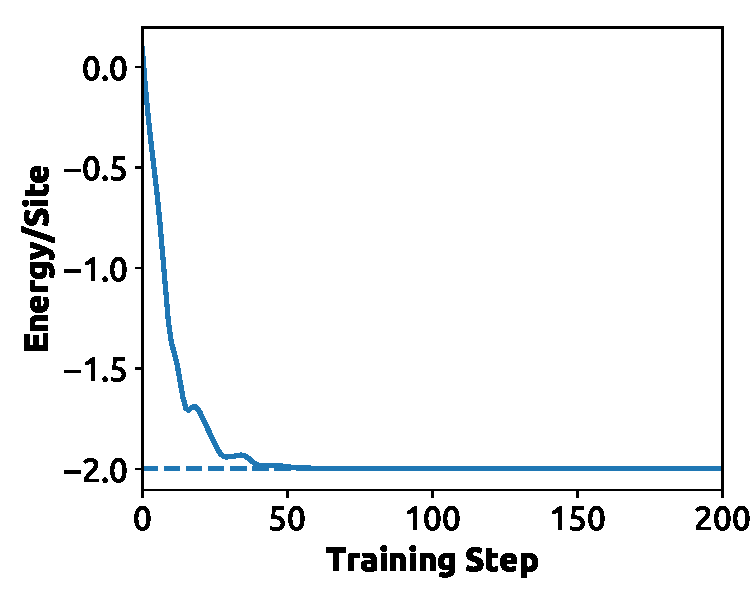
\includegraphics[width=0.5\linewidth,trim={0cm 0cm 0cm 0cm},clip]{images/fig1.pdf}
    \caption{Energy as a function training step. The dashed line corresponds to the exact ground state energy.}\label{fig-qftindex}
\end{figure}

\bibliographystyle{apsrev4-1}
\bibliography{quantum.bib}

\end{document}
